\documentclass{article}

\usepackage{graphicx}
\usepackage{tikz}
\usepackage{tikzsymbols}
\usetikzlibrary{calc,patterns,shapes.geometric}
\pagestyle{empty}
\usepackage[margin=0pt]{geometry}
\geometry{papersize={14in,12in}}

\def\centerarc[#1](#2)(#3:#4:#5){\draw[#1] ($(#2)+({#5*cos(#3)},{#5*sin(#3)})$) arc (#3:#4:#5);}

\begin{document}
	\begin{figure}
		\centering
		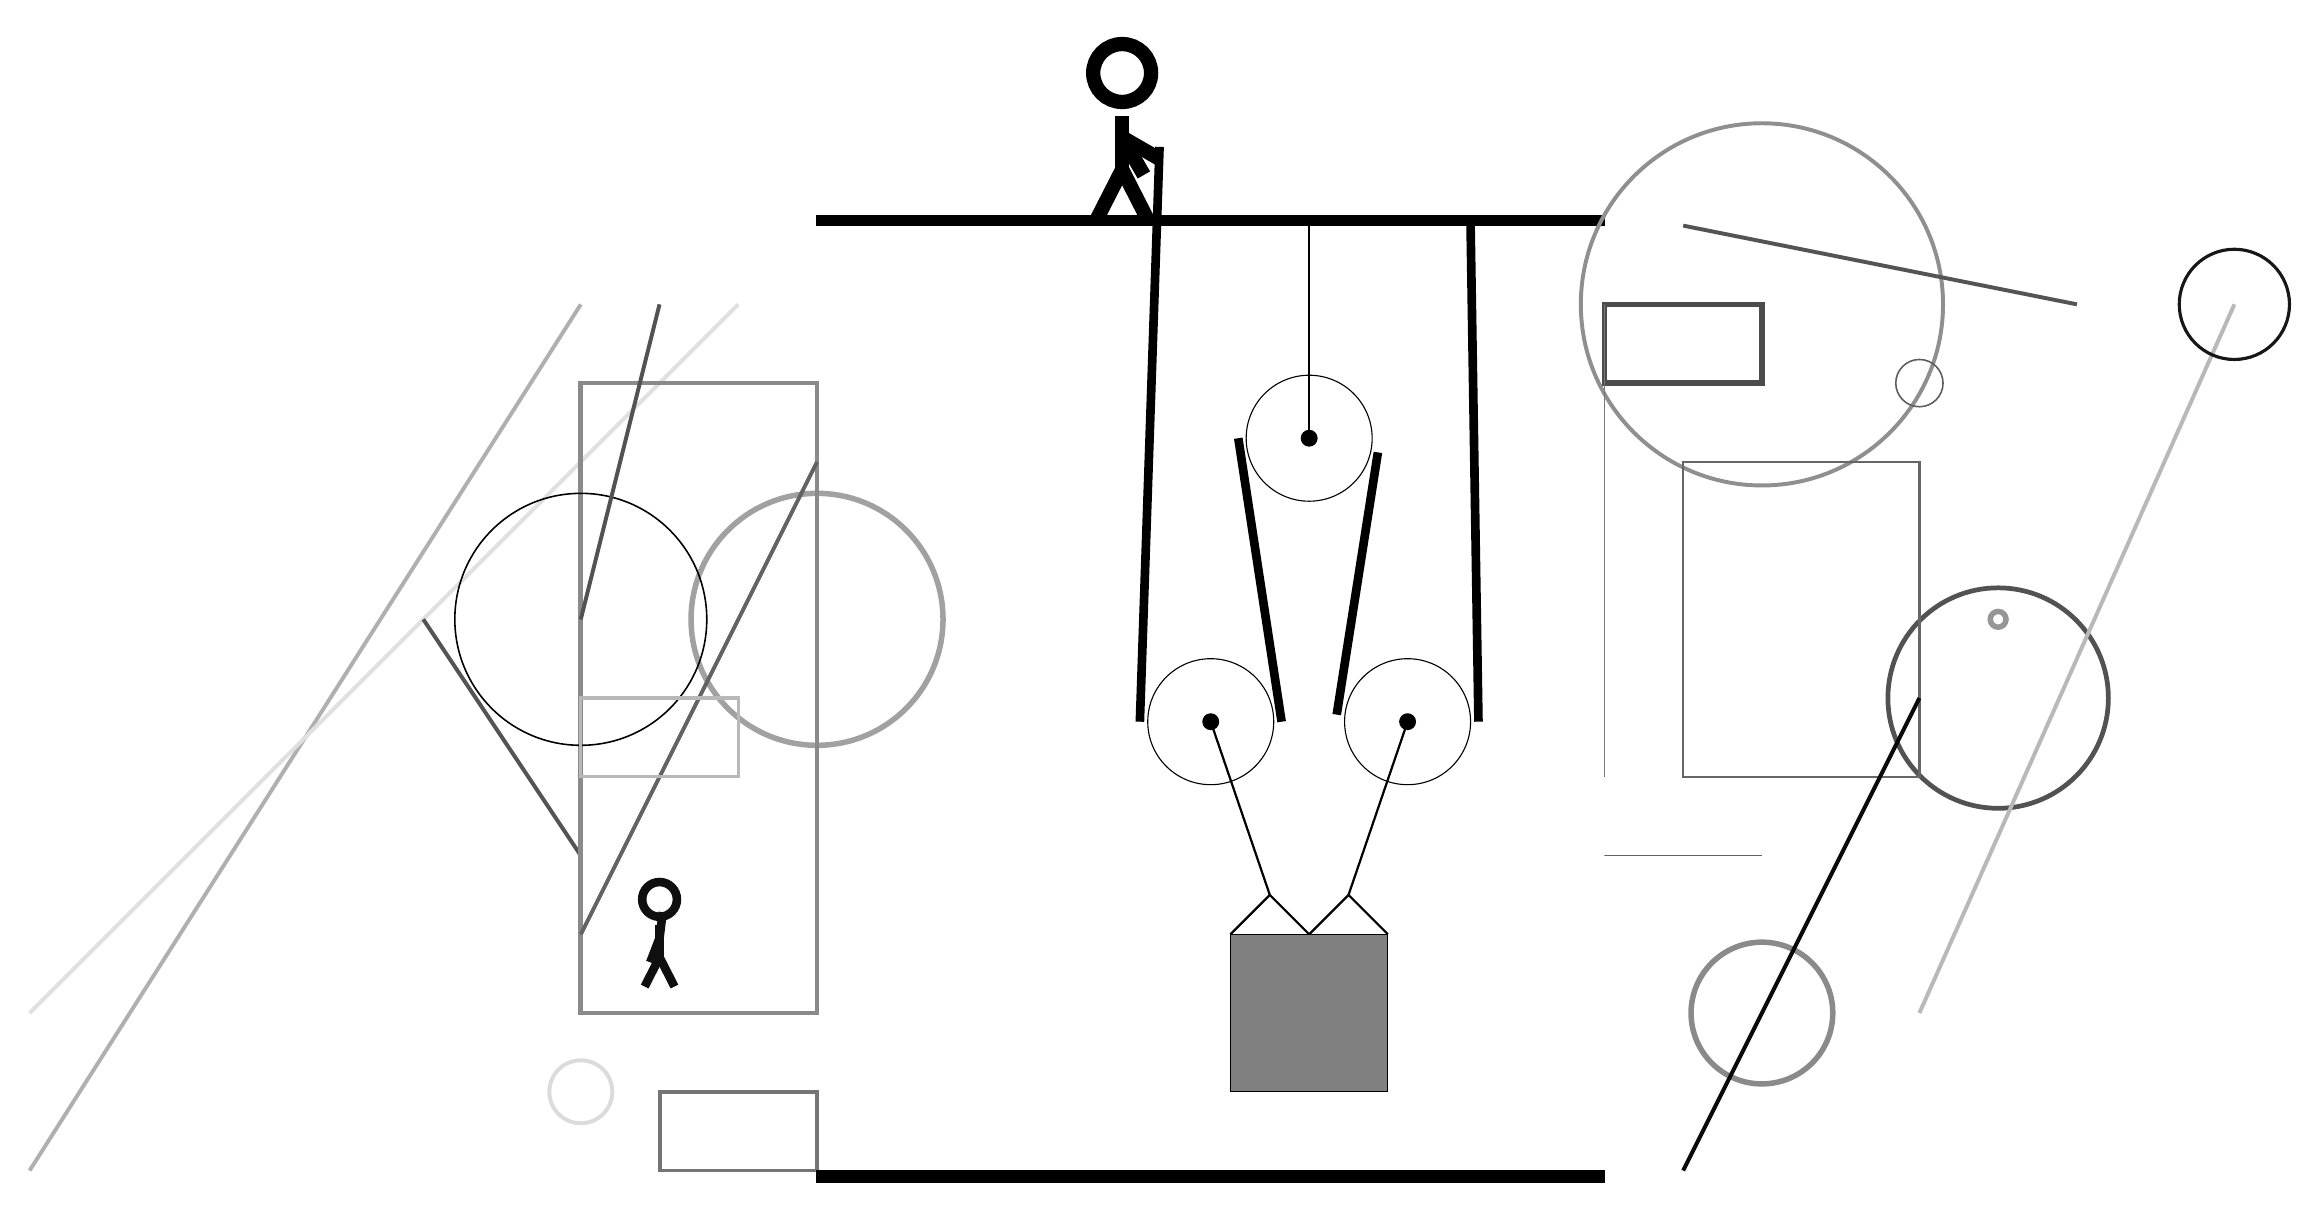
\begin{tikzpicture}
			%%%%% START %%%%%
			
			\draw[fill=black] (-4, 9) rectangle (6, 9.125);
			
			\draw (1, 2.7) circle (0.8);
			\draw[fill=black] (1, 2.7) circle (0.1);
			
			\draw (2.25, 6.3) circle (0.8);
			\draw[fill=black] (2.25, 6.3) circle (0.1);
			\draw[thick] (2.25, 6.3) -- (2.25, 9);
			
			\draw (3.5, 2.7) circle (0.8);
			\draw[fill=black] (3.5, 2.7) circle (0.1);
			
			\draw[thick] (3.5, 2.7) -- (2.75, 0.5);
			\draw[thick] (1, 2.7) -- (1.75, 0.5);
			\draw[thick]  (1.25, 0) -- (1.75, 0.5) -- (2.25, 0);
			\draw[thick]  (2.25, 0) -- (2.75, 0.5) -- (3.25, 0);
			\draw[fill=black!50] (1.25, 0) rectangle (3.25, -2);
			
			\draw [line width=0.7mm, color=black!37](-4, 4) circle (1.6);
			
			\draw [line width=0.5mm, color=black!44](8, 8) circle (2.3);
			\draw [line width=0.6mm, color=black!68](11, 3) circle (1.4);
			\draw[line width=0.5mm, color=black!31](-7, 8) -- (-14, -3);
			\node[line width=0.4mm, color=black!94] at (-6, 0) {\Strichmaxerl[6][69][83]};
			
			\draw[line width=0.5mm, color=black!12](-5, 8) -- (-14, -1);
			\draw[line width=0.3mm, color=black!60] (7, 2) rectangle (10, 6);
			\draw[line width=0.5mm, color=black!67](-9, 4) -- (-7, 1);
			\draw[line width=0.6mm, color=black!46] (-4, 7) rectangle (-7, -1);
			
			\draw [line width=0.5mm, color=black!14](-7, -2) circle (0.4);
			\draw [line width=0.7mm, color=black!46](8, -1) circle (0.9);
			
			\draw[line width=0.5mm, color=black!61](-7, 0) -- (-4, 6);
			\draw[line width=0.5mm, color=black!67](7, 9) -- (12, 8);
			
			\draw[line width=0.5mm, color=black!28](10, -1) -- (14, 8);
			\draw [line width=0.2mm, color=black!100](-7, 4) circle (1.6);
			\draw[line width=0.5mm, color=black!54] (-4, -2) rectangle (-6, -3);
			\draw[line width=0.7mm, color=black!70] (6, 8) rectangle (8, 7);
			\draw[line width=0.2mm, color=black!53] (6, 8) rectangle (6, 2);
			\draw[line width=0.5mm, color=black!68](-6, 8) -- (-7, 4);
			\draw [line width=0.7mm, color=black!41](11, 4) circle (0.1);
			\draw[line width=0.4mm, color=black!28] (-5, 3) rectangle (-7, 2);
			
			\draw[line width=0.2mm, color=black!61] (6, 1) rectangle (8, 1);
			\draw [line width=0.4mm, color=black!91](14, 8) circle (0.7);
			\draw[line width=0.5mm, color=black!96](10, 3) -- (7, -3);
			\draw [line width=0.2mm, color=black!64](10, 7) circle (0.3);
			
			
			\draw[line width=1.1mm] (0.35, 10) --  (0.1, 2.7);
			\centerarc[line width=1.1mm](1, 2.7)(180:360:0.9);
			\draw[line width=1.1mm] (1.9, 2.7) -- (1.35, 6.3);
			\centerarc[line width=1.1mm](2.25, 6.3)(-20:180:0.9);
			\draw[line width=1.1mm](3.123, 6.12) -- (2.6, 2.79);
			\centerarc[line width=1.1mm](3.5, 2.7)(160:360:0.9);
			\draw[line width=1.1mm](4.4, 2.7) -- (4.3, 9);
			
			\node at (-0.07, 10.2) {\Strichmaxerl[10][120][-30]};
			
			\draw[fill=black] (-4, -3) rectangle (6, -3.15);
			
			%%%%% END %%%%%
		\end{tikzpicture}
	\end{figure}	
\end{document}